\documentclass[UTF8,a4paper,12pt,fontset=none]{ctexart}

\usepackage[top=2.54cm,bottom=2.54cm,left=3.17cm,right=3.17cm]{geometry}
\usepackage{setspace}
\setstretch{1.5}

\def\ProjectFontDir{../../fonts}
% Project-local font setup for XeLaTeX.
% Callers may set \ProjectFontDir before \input'ing this file.
\providecommand{\ProjectFontDir}{../fonts}

\setmainfont[
  Path = \ProjectFontDir/tex-gyre/,
  Extension = .otf,
  UprightFont = *-regular,
  BoldFont = *-bold,
  ItalicFont = *-italic,
  BoldItalicFont = *-bolditalic,
  Ligatures = TeX
]{texgyretermes}

\setCJKmainfont[
  Path = \ProjectFontDir/fandol/,
  Extension = .otf,
  BoldFont = FandolSong-Bold,
  ItalicFont = FandolKai-Regular
]{FandolSong-Regular}
\setCJKsansfont[
  Path = \ProjectFontDir/fandol/,
  Extension = .otf,
  BoldFont = FandolHei-Bold,
  ItalicFont = FandolKai-Regular
]{FandolHei-Regular}
\setCJKmonofont[
  Path = \ProjectFontDir/fandol/,
  Extension = .otf,
  ItalicFont = FandolKai-Regular
]{FandolFang-Regular}

\setCJKfamilyfont{zhsong}[
  Path = \ProjectFontDir/fandol/,
  Extension = .otf,
  BoldFont = FandolSong-Bold
]{FandolSong-Regular}
\setCJKfamilyfont{zhsongb}[
  Path = \ProjectFontDir/fandol/,
  Extension = .otf
]{FandolSong-Bold}
\setCJKfamilyfont{zhhei}[
  Path = \ProjectFontDir/fandol/,
  Extension = .otf,
  BoldFont = FandolHei-Bold,
  ItalicFont = FandolKai-Regular
]{FandolHei-Regular}
\setCJKfamilyfont{zhheib}[
  Path = \ProjectFontDir/fandol/,
  Extension = .otf
]{FandolHei-Bold}
\setCJKfamilyfont{zhfs}[
  Path = \ProjectFontDir/fandol/,
  Extension = .otf
]{FandolFang-Regular}
\setCJKfamilyfont{zhkai}[
  Path = \ProjectFontDir/fandol/,
  Extension = .otf
]{FandolKai-Regular}

\ExplSyntaxOn
\cs_if_exist:NT \ctex_punct_set:n
  {
    \ctex_punct_set:n { fandol }
    \ctex_punct_map_family:nn   { \CJKrmdefault         } { zhsong  }
    \ctex_punct_map_family:nn   { \CJKsfdefault         } { zhhei   }
    \ctex_punct_map_family:nn   { \CJKttdefault         } { zhfs    }
    \ctex_punct_map_bfseries:nn { \CJKrmdefault, zhsong } { zhsongb }
    \ctex_punct_map_bfseries:nn { \CJKsfdefault, zhhei  } { zhheib  }
    \ctex_punct_map_itshape:nn  { \CJKrmdefault         } { zhkai   }
  }
\ExplSyntaxOff

\providecommand{\songti}{}
\providecommand{\heiti}{}
\providecommand{\fangsong}{}
\providecommand{\kaishu}{}
\renewcommand{\songti}{\CJKfamily{zhsong}}
\renewcommand{\heiti}{\CJKfamily{zhhei}}
\renewcommand{\fangsong}{\CJKfamily{zhfs}}
\renewcommand{\kaishu}{\CJKfamily{zhkai}}


\usepackage{amsmath}
\usepackage{amsthm}
\usepackage{amssymb}

\usepackage[ruled,linesnumbered]{algorithm2e}
\SetKwComment{Comment}{/* }{ */}
\RestyleAlgo{ruled}

\theoremstyle{definition}
\newtheorem{definition}{定义}

\theoremstyle{plain}
\newtheorem{proposition}{命题}

\theoremstyle{plain}
\newtheorem{lemma}{引理}

\theoremstyle{plain}
\newtheorem{theorem}{定理}

\usepackage{graphicx}
\graphicspath{{./figures/}}
\usepackage{subfig}
\usepackage{color}

\usepackage[backend=biber,style=gb7714-2015,gbpub=false,
            uniquename=init,uniquelist=true,
            maxcitenames=2,mincitenames=1,
            sorting=none]{biblatex}
\addbibresource{refs.bib}

\ctexset{
    section/format = \raggedright\zihao{-4}\heiti\bfseries,
    subsection/format = \raggedright\zihao{5}\heiti\bfseries,
}

\title{面向自动驾驶车辆的梯形棱柱走廊与 B\'{e}zier 曲线时空运动规划}


\author{Srujan Deolasee \and Qin Lin\thanks{通讯作者：Qin Lin (q.lin80@csuohio.edu)} \and Jialun Li \and John M. Dolan}
\date{2022 年 9 月}


\begin{document}

\maketitle

\begin{center}
\vspace{-1em}
\footnotesize
Srujan Deolasee, Birla Institute of Technology and Science, Pilani, Rajasthan, India \\
Qin Lin, Department of Electrical Engineering and Computer Science, Cleveland State University, Cleveland, OH, USA \\
Jialun Li, Dajiang Innovation Technology Co., Ltd, Shenzhen, China \\
John M. Dolan, Robotics Institute, Carnegie Mellon University, Pittsburgh, PA, USA \\[0.3em]
本研究受美国国家科学基金会（National Science Foundation）资助。
\end{center}


%%%%%%%%%%%%%%%%%%%%%%%%%%%%%%%%%%%%%%%%%%%%%%%%%%%%%%%%%%%%%%%%%%%%%%%%%%%%%%%%
\begin{abstract}

具有安全保证的运动规划对自动驾驶车辆生成无碰撞轨迹至关重要。为此，广泛采用路径与速度解耦的分层运动规划方法。在存在动态障碍物的场景下，该方法易出现次优性。时空规划方法同时处理路径规划与速度规划；然而，已有方法仅支持长方体等形状简单的走廊，这在复杂场景中限制了优化的搜索空间。我们提出采用梯形棱柱形走廊进行优化，相较于现有基于长方体走廊的方法，该方案显著扩大了解空间。最后，在所提出的走廊中进行分段 B\'{e}zier 曲线优化。该建模在理论上保证了连续时间轨迹的安全性。我们在数值仿真和 CommonRoad 仿真中验证了所提方法的效率与有效性。
% \srujan{should we mention CommonRoad here?}

\end{abstract}

\noindent\textbf{关键词：}自动驾驶车辆，运动规划，轨迹优化

%%%%%%%%%%%%%%%%%%%%%%%%%%%%%%%%%%%%%%%%%%%%%%%%%%%%%%%%%%%%%%%%%%%%%%%%%%%%%%%%
\section{引言}


%\srujan{introduction- please check once}
运动规划是自动驾驶系统的关键模块之一。在动态交通环境中，运动规划的任务是在考虑无碰撞安全约束、动力学可行性与舒适性的前提下，生成供底层控制器跟踪的轨迹。由于显著不依赖复杂的道路几何结构，Frenet 坐标系 \cite{werling_optimal_2012} 常被用于运动规划。横向运动（沿 $L$ 方向）与纵向运动（沿 $S$ 方向）可以投影到参考线上，参考线通常取为任意形状道路的中心线。再引入时间维度 $T$，即可建立一个便于深入分析与规划的三维 $S − L − T$ 坐标系。

\textbf{路径-速度分离规划（又称分层规划）} 是一种将规划问题分解为两阶段的实用实时方案，即路径规划与速度规划 \cite{gu_runtime-bounded_2016, wenda_xu_real-time_2012, li_real-time_2016}。第一阶段在静态或低速环境中生成路径（$S-L$）。第二阶段在速度规划中生成速度曲线（$S-T$ 或 $L-T$），使自动驾驶车辆能够响应动态障碍物。分层规划的显著缺陷在于，在复杂场景中存在动态障碍物时，容易得到次优解。

\textbf{时空规划} 同时考虑空间与时间维度的机动 \cite{ding_safe_2019, mercy_real-time_2016, ziegler_trajectory_2014}。这种在三维 $S-L-T$ 空间直接优化的方法由于搜索空间更大，通常优于分层规划方法。参见图 \ref{fig:motivation} 所示的启发性示例（将在第 III.A 节中详细讨论）：在涉及横向方向哪怕很小偏离的驾驶场景中，纵向与横向耦合的规划有助于保证全局最优性。%Whereas, the decoupled layered planning approach may result in infeasible trajectories or oscillating behaviour from one time step to another.
%We are motivated by these limitations to perform a direct optimization in the 3D $S-L-T$ space.

\begin{figure}[htbp]
    \centering

    % \subfloat[]{\includegraphics[width=0.21\textwidth]{figures/}\label{fig:f2}}\\
    \subfloat[]{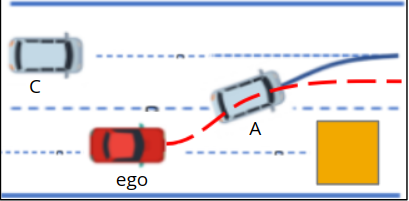
\includegraphics[width=0.32\textwidth, angle=90]{figures/scenario1.png}\label{fig:motivation_a}} \quad\quad
    \subfloat[]{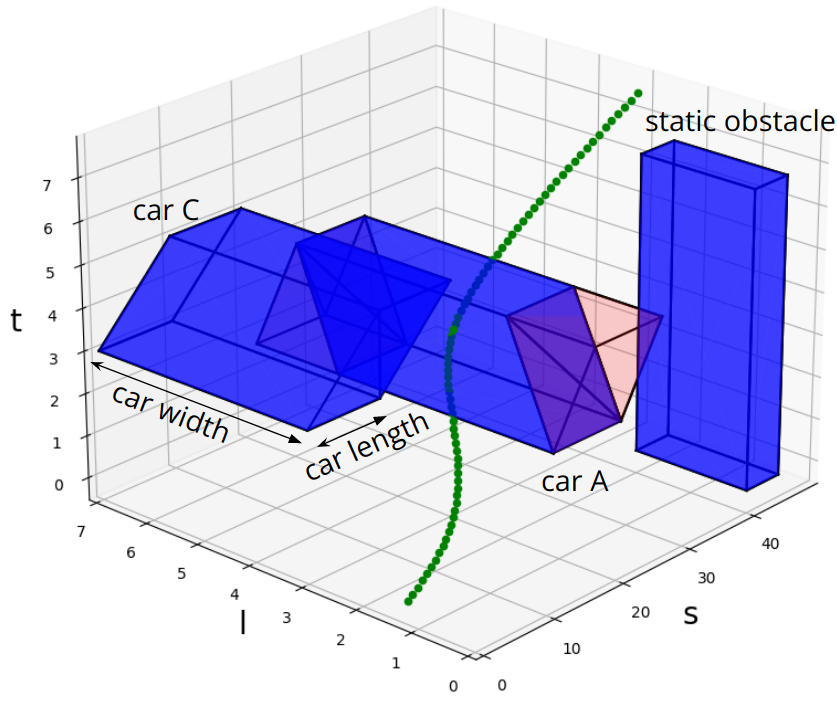
\includegraphics[width=0.32\textwidth]{figures/slt_s1_with_labels.png}\label{fig:motivation_b}}\\
     \subfloat[]{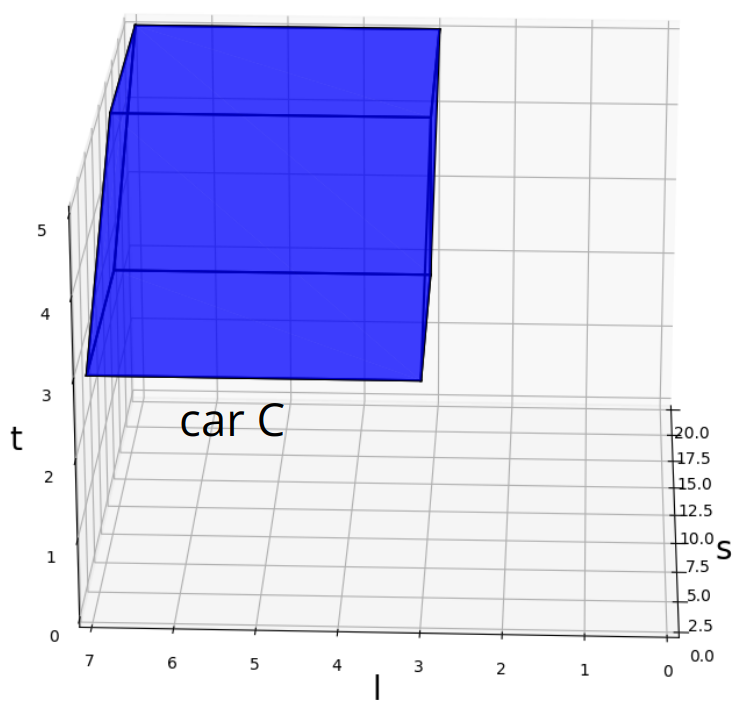
\includegraphics[width=0.32\textwidth]{figures/car_c.png}\label{fig:motivation_c}}
    \subfloat[]{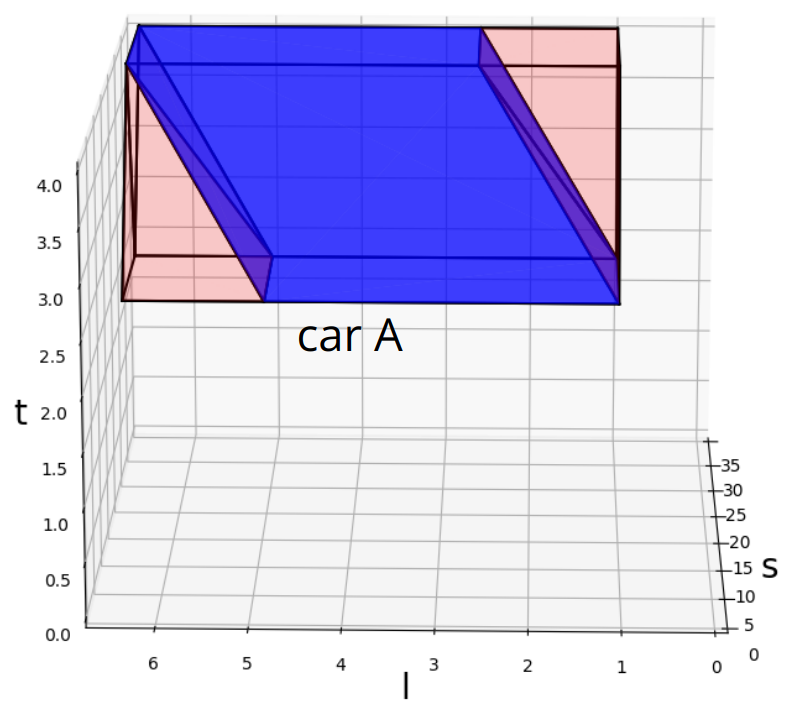
\includegraphics[width=0.32\textwidth]{figures/car_a.png}\label{fig:motivation_d}}
    \caption{让行示例。(a) 鸟瞰图；(b) 我们在三维 $S-L-T$ 图中的时空规划；(c) 从另一视角观察 C 车；(d) 从另一视角观察 A 车。}
    \label{fig:motivation}
\end{figure}

确保安全是运动规划的核心目标。许多已有速度规划方法采用离散时间点施加安全约束。然而，与采样时间无关的、在连续时间空间中可证明的安全保证更为可取。为了解决这一问题，空间走廊被广泛用于轨迹生成。受此启发，我们进一步把空间走廊推广到时空域，以更好地应对动态障碍物。本文利用 B\'{e}zier 多项式的凸包性质，强制连续轨迹始终落在安全的时空区域内。此外，通过所提出的梯形棱柱形走廊，该优化问题的解空间得以扩大。

本文的主要贡献可简述如下：
\begin{enumerate}
    % \item Generate a comfort-optimal trajectory as a reference using the $\ddot{S}-\ddot{L}-T$ graph.
    \item 我们提出一种高效的凸化算法，用于构造由梯形棱柱形走廊组成的三维凸可行区域。
    \item 我们给出 B\'{e}zier 多项式系数的充分条件，从理论上保证轨迹在梯形棱柱走廊中的安全性。与已有的长方体走廊 \cite{ding_safe_2019} 相比，该条件更为宽松，解空间显著扩大，从而提高了找到最优解的可能性。
\end{enumerate}

本文其余部分组织如下。第 II 节回顾相关工作。第 III 节介绍必要的记号与背景材料。第 IV 节给出三维凸安全区域的构造。第 V 节提出优化建模。第 VI 节给出仿真结果与分析。第 VII 节是结论性评述。

\section{相关工作}

\subsection{速度规划}
速度规划技术可分为三类：1) 搜索与优化；2) 采样格并选取最小代价轨迹；3) 近似优化。
\textbf{搜索与优化} 方法在候选速度曲线中搜索最优者，并对曲线进行光顺优化；例见后优化方法 \cite{wenda_xu_real-time_2012}、百度 EM 运动规划器 \cite{fan_baidu_2018} 以及分段急动度速度优化 \cite{zhou_autonomous_2021}。
\textbf{采样} 方法在路径格基础上组合不同的速度格，对生成的局部时空轨迹进行评估，选择代价最小者。相关工作见 \cite{gu_runtime-bounded_2016,wenda_xu_real-time_2012,li_real-time_2016}。前两类方法大多直接在 $S-T$ 图中进行搜索与优化。\textbf{近似优化} 在序列优化问题中考虑车辆动力学模型；例见凸可行集算法 \cite{liu_speed_2017} 以及最优控制方法，如模型预测控制（Model Predictive Control, MPC）\cite{qian_motion_2016} 和约束迭代线性二次调节器（Constrained Iterative Linear Quadratic Regulator, CiLQR）\cite{pan_safe_2020}。这些方法的优点是将动力学模型纳入规划层，缓解了规划与控制的不一致问题；缺点是计算代价较高。

\subsection{自动驾驶车辆的走廊生成}
空间走廊被广泛用于轨迹生成。一些前期工作在静态环境中生成走廊，无法处理动态障碍物 \cite{zhu_convex_2015}, \cite{erlien_safe_2013}。
\citet{liu_convex_2018} 在参考轨迹周围求取凸可行集，但其计算复杂度限制了该方法的实时应用。我们先前的工作提出利用梯形走廊对 $S-T$ 图中的二维空间进行凸化 \cite{li_motion_nodate}。\citet{zhang_sufficient_2022} 给出一种基于通用凸时空走廊的方法。\citet{xu_speed_nodate} 中提出基于改进垂直单元分解的速度规划方法。上述方法均受到前述分层规划固有缺陷的限制。\citet{ding_safe_2019} 采用时空语义走廊（Spatio-Temporal Semantic Corridor, SSC）方法在三维 $S-L-T$ 空间中统一表达障碍物与交通规则。然而，将走廊形状限定为简单长方体，在复杂场景下极大地限制了优化的搜索空间。我们提出的方法将 $S-T$ 中的二维梯形走廊推广到三维 $S-L-T$ 空间，显著扩大了轨迹优化的解空间。由此，我们将空间走廊推广至时空域，以应对动态障碍物，同时满足实时性要求。

\subsection{基于 B\'{e}zier 多项式的规划}

以往，单项式基多项式被用于轨迹生成 \cite{werling_optimal_2012}, \cite{fan_baidu_2018}。然而，这类方法在存在动态障碍物、约束强烈的机动中往往难以表达，并且由于约束只在有限采样点上施加或检查，无法对采样点之间给出安全保证。文献 \cite{gonzalez_speed_2016} 通过恰当的曲线拼接，计算得到光滑连续的速度曲线，但未进行优化且未考虑动态障碍物。B\'{e}zier 多项式与矩形走廊相结合的思想最早起源于无人飞行器（Unmanned Aerial Vehicle, UAV）领域 \cite{gao_online_2018}, \cite{zhou_robust_2019}。\citet{ding_safe_2019} 将其扩展到无人地面车辆（Unmanned Ground Vehicle, UGV）的运动规划。其显著局限在于，所提出的长方体走廊表示无法充分利用自由空间进行优化。在本工作中，我们提出使用时变的梯形棱柱形走廊，并给出将 B\'{e}zier 曲线约束在此类时变走廊中的充分条件以保证安全。理论上可证明，梯形棱柱形走廊能够扩大解空间，从而改善优化效果。

\section{$S-L-T$ 图与轨迹表示}

本节简要介绍 $S-L-T$ 图、B\'{e}zier 多项式以及基于分段 B\'{e}zier 多项式的轨迹表示等背景材料。

\subsection{在 $S-L-T$ 图中表示动态交通参与者}
$S − L − T$ 图在每一时刻表示所有交通参与者的位置，包括过去、当前与预测信息。
以图 \ref{fig:motivation_a} 为例，为简单起见，考虑两辆匀速行驶的车辆。场景描述如下：A 车与自车沿同一车道行驶，该车道上存在一处静态障碍物（例如施工区），两车均需执行换道机动。列举以下典型实体：

 1) \textbf{静态障碍物（六零斜率面型）：} 作为最简单的实体，其六个面的斜率均为零，见图 \ref{fig:motivation_a} 中黄色方块的鸟瞰图以及图 \ref{fig:motivation_b} 中 $S-L-T$ 图的长方体。

 2) \textbf{仅有纵向运动的运动车辆（四零斜率面型）：} C 车直线前行即为一例，见图 \ref{fig:motivation_a}。图 \ref{fig:motivation_b} 中 C 车的顶面与底面斜率为零。其两个侧面（见图 \ref{fig:motivation_c} 中左右侧面的另一视角）垂直于 $S-L$ 平面，无斜率。平行四边形沿 $L$ 轴的边长为车辆宽度加安全区；沿 $S$ 轴的边长为车辆长度加上自车车长的一半作为安全区。

 3) \textbf{同时存在纵向与横向运动的运动车辆（二零斜率面型）：} 例如图 \ref{fig:motivation_a} 中向左前方行驶的 A 车。如图 \ref{fig:motivation_b} 所示，仅顶面与底面斜率为零。


 $S-L-T$ 图中的三维自由空间一般是非凸的。我们提出对 \emph{二零斜率面型} 的平行六面体进行过近似，使其成为 \emph{四零斜率面型} 的平行六面体，例如图 \ref{fig:motivation_b} 中 A 车对应的粉色膨胀空间（见图 \ref{fig:motivation_b} 与图 \ref{fig:motivation_d}）。这样做具有两大优势：1) 在存在此类平行六面体的情况下，我们将证明可以把二维走廊构造算法 \cite{li_motion_nodate} 高效地扩展为三维梯形棱柱形走廊的构造；2) 尽管过近似会损失部分空间，安全走廊仍显著大于目前最先进的长方体走廊。需要指出的是，本文方法中二维与三维之间的变换不会损失搜索空间。综上，我们在精确性与效率之间取得良好折衷。过近似步骤所选择的面由该过程中损失的搜索空间体积最小化来确定。直观地，如果车辆的横向速度小于纵向速度，则对应面被选作过近似。

\subsection{B\'{e}zier 多项式及其性质}

B\'{e}zier 多项式是由 Bernstein 基的线性组合所表示的多项式函数。$n$ 阶 B\'{e}zier 多项式可写作
$$
B(t)=c_{0} b_{n}^{0}(t)+c_{1} b_{n}^{1}(t)+\cdots+c_{n} b_{n}^{n}(t)=\sum_{i=0}^{n} c_{i} b_{n}^{i}(t)
$$
其中 Bernstein 基满足 $b_{n}^{i}(t)=C_{i}^{n} \cdot t^{i} \cdot(1-$ $t)^{n-i}, t \in[0,1]$。多项式系数 $c_{i}(i=$ $0,1, \ldots, n$) 亦称为控制点。与单项式多项式相比，B\'{e}zier 曲线具有如下性质：


\begin{itemize}
    \item 时间区间定义在 $t \in[0,1]$ 上。
    \item B\'{e}zier 多项式起于控制点 $B(0)=c_{0}$，止于 $B(1)=c_{n}$。
    \item 凸包性质：B\'{e}zier 曲线 $B(t)$ 始终位于控制点的凸包之内。
    \item 速矢端线性质：由速矢端线性质，$B(t)$ 的导数 $\dot{B}(t)$ 也可写为 B\'{e}zier 多项式，其控制点为 $c_{i}^{1}=n \cdot\left(c_{i+1}-c_{i}\right), i=$ $0,1, \ldots, n-1$。对导数 B\'{e}zier 曲线应用凸包性质，可将原曲线 $B(t)$ 的整个动力学分布约束在给定的动力学范围内。
\end{itemize}

\subsection{基于 B\'{e}zier 多项式的轨迹表示}
为了缓解数值不稳定问题，我们用较低阶的分段 B\'{e}zier 多项式取代对整个规划时域使用单一高阶 B\'{e}zier 多项式。轨迹的每一段对应一个梯形棱柱走廊。注意 $B(t)$ 定义在固定时间区间 $[0,1]$ 上。对于由 $m+1$ 段组成的整条轨迹，在每一段 $\left[T_{k}, T_{k+1}\right] (k = 0,1,\ldots,m)$ 上，我们在时域上采用尺度变换与平移变换将其映射到区间 $[0,1]$ [13]。于是，整条分段轨迹在某一维 $\sigma\in\{s,l\}$ 上可写为
$$
f^{\sigma}(t)=\left\{\begin{array}{c}
h_{0} B_{0}\left(\frac{t-T_{0}}{h_{0}}\right), t \in\left[0, T_{1}\right] \\
h_{1} B_{1}\left(\frac{t-T_{1}}{h_{1}}\right), t \in\left[T_{1}, T_{2}\right] \\
\vdots \\
h_{m} B_{m}\left(\frac{t-T_{m}}{h_{m}}\right), t \in\left[T_{m}, T_{m+1}\right] .
\end{array}\right.
$$
其中 $h_i$ 为尺度变换因子，$T_i$ 为平移变换因子，$i = 0,1,\ldots,m$，且 $T_0 = 0$。


\section{走廊生成}

本节介绍一种凸化算法，用于将原有的非凸优化问题转化为凸走廊形式以便实时求解。为优化过程提供热启动通常依赖参考轨迹。本工作中采用简单的分段函数，在自车的位形空间中生成有效的参考路径点。

\subsection{分段凸安全区域的表示}

设整个安全区域被划分为 $m+1$ 段，对应时间区间 $\left[T_{0}, T_{1}\right], \ldots,\left[T_{m}, T\right]$ 且 $T =T_{m+1}$，每一区间对应一个凸安全区域。此类凸化算法的细节将在下一节介绍。$S-L-T$ 空间中第 $k$ 个凸安全区域可表示为
$$\mathcal{S}_{k} = \{\ (t_i, s_i, l_i)\ | $$
$$\underline{p^{k}_0} + h_k \underline{p^{k}_1} \frac{t_i - T_k}{h_k} \leq s_i \leq \overline{p^{k}_0} + h_k \overline{p^{k}_1} \frac{t_i - T_k}{h_k},$$
$$l_{beg} \leq l_i \leq l_{end},\ t_i \in [T_k, T_{k+1}]\ \}$$
% $$\mathcal{S}_{k} = \{\ (t_i, s_i, l_i)\ | $$
% $$\underline{p^{k}_0} + h_k \underline{p^{k}_1} \frac{t_i - T_k}{h_k} \leq s_i \leq \overline{p^{k}_0} + h_k \overline{p^{k}_1} \frac{t_i - T_k}{h_k},$$
% $$l_{beg} \leq l_i \leq l_{end},$$
% $$ t_i \in [T_k, T_{k+1}]\ \}$$
其中 $s_i$ 与 $l_i$ 分别为第 $i$ 个控制点的纵向与横向坐标，$\underline{p_{0}^{k}}, \underline{p_{1}^{k}}$ 为下界的偏置与斜率，$\overline{p_{0}^{k}}, \overline{p_{1}^{k}}$ 为上界的偏置与斜率。$h_{k}$ 表示第 $k$ 个时间区间的长度，满足 $h_{k}=T_{k+1}-T_{k}, k=0,1, \ldots, m$。

于是，整个安全区域为一组分段安全子区域之并：$
\mathcal{S}=\mathcal{S}_{0} \cup \cdots \cup \mathcal{S}_{m}$。若 $\forall t_{0} \in[0, T], s\left(t_{0}\right) \in \mathcal{S}, l\left(t_{0}\right) \in \mathcal{S}$，则速度规划是安全的，这等价于对 $t_{0} \in\left[T_{k}, T_{k+1}\right]$ 有 $s\left(t_{0}\right) \in \mathcal{S}_{k}, l\left(t_{0}\right) \in \mathcal{S}_{k}, k=0,1, \ldots, m$，即
$$
\underline{p_{0}^{k}}+h_{k} \underline{p_{1}^{k}} \frac{t_{0}-T_{k}}{h_{k}} \leq s\left(t_{0}\right) \leq \overline{p_{0}^{k}}+h_{k} \overline{p_{1}^{k}} \frac{t_{0}-T_{k}}{h_{k}}
$$
$$
l_{beg} \leq l\left(t_{0}\right) \leq l_{end}
$$

\subsection{分段凸安全区域的构造}
\begin{figure}[htbp]
    \centering
    \subfloat[$S-L-T$ 图]{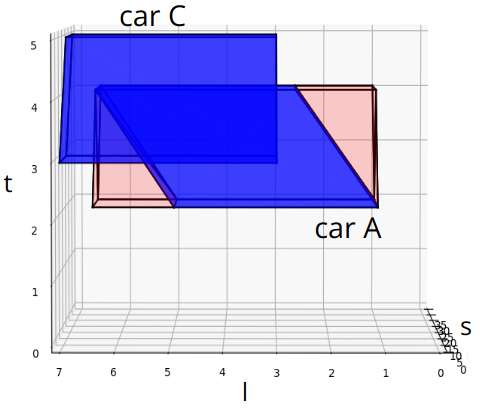
\includegraphics[width=0.32\textwidth]{figures/scene1_car_ac.png}\label{fig:f5}} \quad\quad
    \subfloat[过近似（红色）]{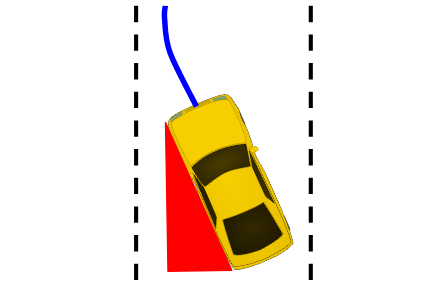
\includegraphics[width=0.35\textwidth]{figures/over_approximation_large.png}\label{fig:f5.5}}\\
    % \subcaption{result of over-approximation}
    \subfloat[$l \in [1,3)$ 处的 $S-T$ 图]{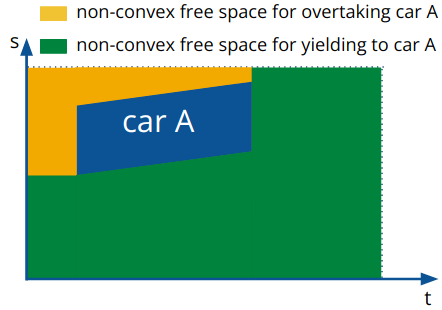
\includegraphics[width=0.32\textwidth]{figures/s_t_cross_sections/homotopy_st_1.png}\label{fig:f7}}\quad
    \subfloat[$l \in [3,6.7)$ 处的 $S-T$ 图]{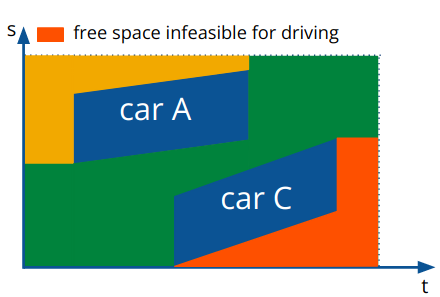
\includegraphics[width=0.32\textwidth]{figures/s_t_cross_sections/homotopy_st_2.png}\label{fig:f6}}
    \caption{在对 A 车进行过近似后，图 \ref{fig:motivation_b} 中的场景}
    \label{fig:Fig 2}
    % \srujan{please check the updated figures}
\end{figure}
算法 1 概述了三维梯形走廊的生成过程。在 $S-L-T$ 图中，沿 $L$ 轴在任一障碍物的起始或终止 $L$ 坐标处对原非凸空间进行切片。由此得到的非凸空间的三维块可被投影到二维 $S-T$ 图中而 \textit{不会} 损失任何搜索空间。例如，在图 \ref{fig:f5} 中，任何位于 $[1,3)$ 范围内的 $L$ 切片都会给出如图 \ref{fig:f7} 所示的二维 $S-T$ 横截面。类似地，任何位于 $[3, 6.7)$ 的 $L$ 切片都会给出如图 \ref{fig:f6} 所示的 $S-T$ 图。算法 1 的输入为自车与道路在 $S$ 与 $L$ 方向上的上下界，这些界在时间时域上以离散时间间隔 $\Delta$ 测量得到。

对于每个切片，我们在相应的 $S-T$ 图中构造二维凸走廊。本文在前期工作 \cite{li_motion_nodate} 中的二维凸梯形走廊生成算法基础上进行推广，新的算法作为算法 2 给出。

算法 2 概述了在沿 $L$ 轴给定的任意 $S-T$ 横截面内构造二维分段凸安全区域的过程。$S$ 方向的上下界作为该算法的输入。算法 2 的具体运行细节请读者参阅 \cite{li_motion_nodate}。
本文的一个关键改动在于：在子程序 $SingleRegionCaculate()$ 中，我们同时初始化区域在 $L$ 方向上的上下边界（算法 3 第 6、7 行）。我们的过近似步骤以及算法 1 的设计保证了算法 2 生成的所有二维凸区域在这两个边界上保持一致。因此，本质上我们获得了沿 $L$ 轴 \textit{拖拽} 而成的二维梯形走廊，从而形成三维梯形棱柱形凸走廊。最后，$RegionSplit()$ 用于检查每个二维凸区域的长度。若其超过用户设定的阈值（例如在我们的实验设置中为 $1\ s$），则将其切分为若干子区域，各子区域的时间间隔均低于该阈值。该细化操作旨在避免欠拟合。

这一二维走廊生成过程针对 $S-L-T$ 图中所有不同的障碍物边界重复进行（算法 1 第 1 行）。沿 $L$ 轴对边界的初始化保证了所得到的是三维梯形凸走廊。由于走廊在 $L$ 方向的长度由 $S-L-T$ 空间中障碍物的起始或终止给定，我们可以保证算法 1 所生成的所有走廊的安全性。注意，对于由障碍物划分的空间，我们通过 $SelectCorridors()$ 方法选出唯一包围参考轨迹的那部分空间。为了对 A 车让行，根据三维参考路径点，选取位于图 \ref{fig:f7} 和图 \ref{fig:f6} 中绿色区域内的走廊。
注意，一旦选定走廊，整个优化即作为一个整体问题求解，而不是分解为针对各个走廊的独立子优化。




\begin{algorithm}[htbp]
\caption{Piecewise 3D Convex Regions Generation}
%\SetAlgoLined
\setcounter{AlgoLine}{0}
\LinesNumbered
\KwIn{$obs, lb_s[obs], up_s[obs], lb_l[obs], up_l[obs], nums, \Delta$}

\KwOut{3D\_Region}

$\textbf{Initialize:}$ \For{$i \gets 0 \textbf{ to } obs$}{
    $corridor = Convexify2D(lb_s[i], ub_s[i], lb_l[i], ub_l[i], nums, \Delta)$;

    $new\_corridor.append(corridor)$;
}
$final\_corridor = SelectCorridors(new\_corridor)$;

$\textbf{Return } final\_corridor$
\end{algorithm}


\begin{algorithm}[htbp]
\small
\caption{Convexify2D}\label{alg:two}
\setcounter{AlgoLine}{0}
\LinesNumbered
\KwIn{ $lb_s, ub_s, lb_l, ub_l, nums, \Delta$}

\KwOut{ $regions$}

$\textbf{Initialize: } regions[0], i = 0, j = 1$ \Comment{i 与 j 分别为元片和结果凸区域的计数器}
$SingleRegionCalculate(region,0,lb_s[0],ub_s[0],lb_s[1],$\\\ \ $ub_s[1], lb_l, ub_l)$\\
$regions.append(region)$
\\
\For{$i \gets 2 \textbf{ to } nums-1$}{
$lskew = (lb_s[i] - lb_s[i-1])/\Delta$ \Comment{相邻两元片的下界斜度}
$uskew = (ub_s[i]-ub_s[i-1])/\Delta$ \Comment{上界斜度}
     \If{$||lskew-regions[j-1].lskew|| > \epsilon \textbf{ or } ||uskew-regions[j-1].uskew|| > \epsilon$}{
    $regions[j-1].t_{end} = i$\\
    $regions[j-1].t = (regions[j-1].t_{end}-regions[j-1].t_{beg})*\Delta$\\
    $SingleRegionCalculate(region,j,lb_s[i],ub_s[i],$\\\ \ $lb_s[i+1],ub_s[i+1], lb_l, ub_l)$\\
    $regions.append(region)$\\
    $j \gets j+1$
  }
}
$regions[j-1].t_{end} = nums-1$\\
$regions[j-1].t = (regions[j-1].t_{end} - regions[j-1].t_{beg})*\Delta$\\
$RegionSplit(regions)$\\
% $RegionMerge(regions)$\\
\textbf{Return} {$regions$}
\end{algorithm}
%\vespace{-5cm}
\begin{algorithm}[htbp]
\caption{Single Region Caculate}
\setcounter{AlgoLine}{0}
\LinesNumbered
\KwIn{ $region,j,lb_s[i],ub_s[i],lb_s[i+1],ub_s[i+1], lb_l, ub_l$}
\KwOut{ $region$} %\Comment{updated region}
 $region.t_{beg} = j$\\
 $region.lskew = (lb_s[i + 1] - lb_s[i])/\Delta$\\
 $region.lbias = lb_s[i]$\\
 $region.uskew = (ub_s[i + 1] - ub_s[i])/\Delta$\\
 $region.ubias = ub_s[i]$\\
 $region.l_{beg} = lb_l$\\
 $region.l_{end} = ub_l$\\
\end{algorithm}

\section{分段 B\'{e}ZIER 多项式优化}
在本节中，我们进一步讨论使用长方体走廊的局限性，随后讨论梯形棱柱形走廊中的安全约束，最后介绍基于新设计的凸解空间的二次优化建模。

\subsection{长方体走廊安全约束的局限性}
如第 III.C 节所述，B\'{e}zier 曲线的凸包性质被用于强制使 $S-L-T$ 图中的轨迹停留在安全区域 $\mathcal{S}$ 内。我们首先正式定义用于轨迹生成的走廊：

\begin{definition}
\textit{设 B\'{e}zier 多项式的系数为 $c_i \in \Omega, i=0,1,\ldots,n$，每个控制点有两个维度 $\{S, L\}$。位于安全区域 $\mathcal{S}$ 内的这些控制点构成子集 $\mathcal{S}^{cor} \subseteq \mathcal{S}$，称为走廊。}
\end{definition}

\citet{ding_safe_2019} 在 $S-L-T$ 图中给出了长方体走廊的构造。长方体走廊对控制点的约束由以下命题给出：

\begin{proposition}
若一条轨迹在每个时间区间上的控制点满足 $c^{k}_i \in \Omega^{k}_{cub} = \{c^k | \underline{p_{0}^{k}}+h_{k} \underline{p_{1}^{k}} \leq c^{k,s} \leq \overline{p_{0}^{k}}, l^{k}_{beg} \leq c^{k,l} \leq l^{k}_{end}, i=0,1,\ldots,n, k=0,1,\ldots,m\}$，则 $f(t)$ 可被保证是安全的，且其上下界构成长方体走廊 $\mathcal{S}^{cub}$。
\end{proposition}
% \begin{Proof}
关于矩形走廊中安全约束的证明见 \cite{li_motion_nodate}，并可直接推广到第三维 $L$ 得到长方体走廊的情形。
% Hence, we skip the proof for brevity.
% \end{Proof}

%The problem of using cuboidal corridors in the $S-L-T$ graph is that when the bounds of corridors in the $S$ direction meet $\underline{p}_{0}^{k}+h_{k} \underline{p_{1}^{k}}>\overline{p_{0}^{k}}$, there is no feasible solution of the optimization problem and the planner will fail. In order to avoid this case, the time intervals of the $k$-th corridors should satisfy $h_{k} \leq \frac{\overline{p_{0}^{k}}-p_{0}^{k}}{\underline{p_{1}^{k}}}$.

当任一下界（$\underline{p}_{0}^{k}+h_{k} \underline{p_{1}^{k}}$）大于上界（$\overline{p_{0}^{k}}$）时，优化失败。为了避免这种情形，第 $k$ 个走廊的时间间隔必须满足 $h_{k} \leq \frac{\overline{p_{0}^{k}}-p_{0}^{k}}{\underline{p_{1}^{k}}}$。

\citet{ding_safe_2019} 提出了一种种子生成与立方体膨胀方法来调整时间间隔。然而，该方法会产生大量走廊和优化变量，导致计算代价较高。%In addition, if $\exists \  \underline{p_{1}^{k}} > 0$ or $\overline{p_{1}^{k}} > 0$ the cuboidal corridors fail to cover all the safe regions. As a result, the search space is sub-optimal and the constraints on control points to enforce the trajectory in cuboidal corridors are overtightened.
在常见驾驶场景中（图 \ref{fig:motivation}），我们有 $\underline{p_{1}^{k}} > 0$ 或 $\overline{p_{1}^{k}} > 0$，因而长方体走廊无法覆盖所有安全区域。结果使搜索空间次优，施加在控制点上的约束%in cuboidal corridors
也被过度收紧。
%(see the illustrations in Fig. 3(a) and 3(c) for examples of this in 2D).
%In the next subsection, we will introduce the safety enforcement for our proposed trapezoidal-prism corridors with enlarged solution space.

\subsection{梯形棱柱走廊中的安全约束}
使纵向与横向轨迹同时安全并落在所提出的梯形棱柱走廊内的控制点 $c_i$ 的充分条件，建立在以下引理之上。

\begin{lemma}
设 $M \in \mathbb{R}^{(n+1) \times(n+1)}$ 为从 Bernstein 基 $\left\{b_{n}^{0}(t), b_{n}^{1}(t), \ldots, b_{n}^{n}(t)\right\}$ 到单项式基 $\left\{1, t, t^{2}, \ldots, t^{n}\right\}$ 的转移矩阵。则有 $M_{i, 0}=1,0 \leq$ $M_{i, j} \leq 1, i=0,1, \ldots, n, j=0,1, \ldots, n$。
\end{lemma}
证明见 \cite{li_motion_nodate}。我们利用下述针对二维梯形走廊的定理，构造三维梯形棱柱形走廊。
\begin{theorem}
对一条轨迹，若在每个时间区间上其控制点满足 $c_{i}^k \in \Omega^k$，其中 $\Omega^k = \{c^k | \underline{p_{0}^{k}}+h_{k}\underline{p_{1}^{k}}M_{i,1} \underline{p_{1}^{k}} \leq c_{i}^{k,s} \leq \overline{p_{0}^{k}}+h_{k}\overline{p_{1}^{k}}M_{i,1}, l^{k}_{beg} \leq c_{i}^{k,l} \leq l^{k}_{end}, i=0,1,\ldots,n,k=0,1,\ldots,m\}$，则 $f(t)$ 可被保证是安全的。$S$ 和 $L$ 方向的上下界共同构成梯形棱柱形走廊 $\mathcal{S}^{trp}$。
\end{theorem}
上述定理在二维情形下的证明见 \cite{li_motion_nodate}，可直接推广到另一维度 $L$。
% Hence, we skip the proof for brevity.

在定理 1 中，$c_{i}^{s}$ 的约束为 $\underline{p_{0}^{k}}+h_{k}\underline{p_{1}^{k}}M_{i,1} \underline{p_{1}^{k}} \leq c_{i}^{k,s} \leq \overline{p_{0}^{k}}+h_{k}\overline{p_{1}^{k}}M_{i,1}$。相较于命题 1 给出的长方体走廊安全约束，有 $\underline{p_{0}^{k}}+h_{k}\underline{p_{1}^{k}}M_{i,1} \leq \underline{p_{0}^{k}}+h_{k} \underline{p_{1}^{k}}$ 及 $\overline{p_{0}^{k}}+h_{k}\overline{p_{1}^{k}}M_{i,1} \geq \overline{p_{0}^{k}}$。采用梯形走廊的优势有两方面：i) 根据 $\underline{p_{0}^{k}}+h_{k}\underline{p_{1}^{k}}M_{i,1} \underline{p_{1}^{k}} \leq c_{i}^{k,s} \leq \overline{p_{0}^{k}}+h_{k}\overline{p_{1}^{k}}M_{i,1}$ 的证明，下界始终不大于上界；而对于矩形走廊，我们必须始终检查 $h_{k} \leq \frac{\overline{p_{0}^{k}}-p_{0}^{k}}{\underline{p_{1}^{k}}}$；ii) 约束得到放松，因此解空间更大，从而更有可能获得最优解。

\subsection{轨迹优化建模}
目标函数建立为
\begin{equation}
 \begin{aligned}
&J = J_s + J_l\\
&J_s = w_{1} \int_{0}^{T}\left(s(t)-s^{r}(t)\right)^{2} \mathrm{~d} t+w_{2} \int_{0}^{T}\left(\dot{s}(t)-v_{s}^{r}\right)^{2} \mathrm{~d} t \\
&+w_{3} \int_{0}^{T} \ddot{s}(t)^{2} \mathrm{~d} t+w_{4} \int_{0}^{T} \dddot{s}(t)^{2} \mathrm{~d} t+w_{5}\left(s(T)-s^{r}(T)\right)^{2}\\
&J_l = w_{6} \int_{0}^{T}\left(l(t)-l^{r}(t)\right)^{2} \mathrm{~d} t+w_{7} \int_{0}^{T}\left(\dot{l}(t)-v_{l}^{r}\right)^{2} \mathrm{~d} t \\
&+w_{8} \int_{0}^{T} \ddot{l}(t)^{2} \mathrm{~d} t+w_{9} \int_{0}^{T} \dddot{l}(t)^{2} \mathrm{~d} t+w_{10}\left(l(T)-l^{r}(T)\right)^{2}\\
\end{aligned}
\end{equation}
其中 $s^{r}(t)$ 和 $l^{r}(t)$ 为参考纵向轨迹与参考横向轨迹，$v^{r}_s$ 和 $v^{r}_l$ 为两个方向的参考速度。对于 $J_s$ 和 $J_l$，第一项惩罚对参考轨迹的偏差；第二项惩罚实际速度与参考速度的偏差；第三、四项分别惩罚加速度和急动度；最后一项惩罚终点位置与参考终点的偏差。我们使用 Optuna\cite{optuna_2019} 对这 10 个参数进行调优。%for one scenario. These weights were further adjusted manually to solve the optimization of all the various scenarios tested.

优化考虑以下约束：
\begin{itemize}
    \item 边界约束：分段曲线从固定的位置、速度与加速度起始，即
    $$
    c_{i}^{0, l} h_{k}^{(1-l)}=\left.\frac{\mathrm{d}^{l} f(t)}{\mathrm{d} t^{l}}\right|_{t=0}, \quad l=0,1,2,
    $$
    其中 $c_{i}^{k, l}$ 是第 $k$ 条 B\'{e}zier 曲线 $l$ 阶导数的控制点。注意 $c_{i}^{k, l}$ 具有 $\{S,L\}$ 两个维度。
    \item 连续性约束：分段曲线在连接时刻处的位置、速度与加速度必须连续。
    $$
    c_{n}^{k, l} h_{k}^{(1-l)}=c_{0}^{k+1, l} h_{k+1}^{(1-l)}, l=0,1,2, k=0,1, \ldots, m-1
    $$
    \item 安全约束：在所提出的梯形棱柱走廊中，控制点纵向分量的安全约束可写为
    $$
    \underline{p_{0}^{k}}+h_{k} \underline{p_{1}^{k}} M_{i, 1} \leq c_{i}^{k, 0} \leq \overline{p_{0}^{k}}+h_{k} \overline{p_{1}^{k}} M_{i, 1}, k=0,1, \ldots, m
    $$
    控制点横向分量的安全约束为
    $$
    l_{beg} \leq c_{i}^{k, 0} \leq l_{end}
    $$
    \item 物理约束：物理约束包括对车辆速度、加速度和急动度的限制。我们可以利用 B\'{e}zier 曲线的速矢端线性质计算速度、加速度和急动度。约束为
    $$
    \begin{aligned}
    \beta^{k, 1} & \leq c_{i}^{k, l} \leq \overline{\beta^{k, 1}} \\
    \beta^{l} & \leq c_{i}^{k, l} \leq \overline{\beta^{l}}, l=2,3
    \end{aligned}
    $$
    其中 $k=0,1, \ldots, m$，且 $c_{i}^{k, l+1}=(n-$ $l)\left(c_{i+1}^{k, l}-c_{i}^{k, l}\right)$。上界 $\overline{\beta^{k, 1}}$ 由道路限速和向心加速度约束决定。设 $a_{c m}$ 为允许的最大加速度，$\kappa_{k}$ 为 $t \in\left[T_{k}, T_{k+1}\right]$ 时段内路径的最大曲率（详见 \cite{8916917}）。横向加速度约束为
    $$
    c_{i}^{k, l} \leq \overline{\beta^{k, 1}}=\sqrt{\frac{a_{c m}}{\kappa_{k}}} .
    $$
各段速度曲线的纵向、横向加速度与急动度的界相同。
\end{itemize}
于是，轨迹优化过程可建模为二次规划（Quadratic Programming, QP）问题：
    $$
    \begin{aligned}
    \mathbf{P}:  \quad \min _{\mathbf{c}} \ & \frac{1}{2} \mathbf{c}^{T} \mathbf{Q}_{\mathbf{c}} \mathbf{c}+\mathbf{q}_{\mathbf{c}}^{T} \mathbf{c}+\mathrm{const} \\
    \text { s.t. } & \mathbf{A}_{e q} \mathbf{c}=\mathbf{b}_{e q} \\
    & \mathbf{A}_{i e} \mathbf{c} \leq \mathbf{b}_{i e} .
    \end{aligned}
    $$
具体建模过程请读者参阅我们前期工作的附录 \cite{extended}。该问题可由诸如 OSQP\cite{osqp} 等现代求解器实时求解。

\section{仿真与结果分析}
% \subsection{Implementation Details}
%The experiments done to validate our approach assume that the poses of the surrounding vehicles can be predicted.
我们的框架采用 C++11 实现。所有仿真均在一台配备 2.60GHz Intel i10-10750H 处理器的个人计算机上进行。
\subsection{数值仿真}
我们通过数值仿真将所提方法与长方体走廊方法 \cite{ding_safe_2019} 进行比较。规划时域为 7 s。不同的道路场景如下：

\subsubsection{因道路施工并入另一车道} 考虑图 \ref{fig:motivation} 所示场景。我们将车辆的不同位置投影到 $S-L-T$ 图上。自车的初始速度和加速度分别为 $v_{s}(0) = 7.0\ \textnormal{m/s}, v_{l}(0) = 0\ \textnormal{m/s}$ 和 $a_{s}(0) = 0\ \textnormal{m/s\textsuperscript{2}}, a_{l}(0) = 0\ \textnormal{m/s}\textsuperscript{2}$。
% The parameters for $J_s$ are set to be $w1 = 0.0, w2 = 0.1, w3 = 20.0, w4 = 10.0$ and $w5 = 3.0$, and those for $J_l$ are set to be $w2 = 0.1, w2 = 0.0, w3 = 10.0, w4 = 5.0$ and $w5 = 3.0$.

\begin{figure}[htbp]
    \centering
    \subfloat[]{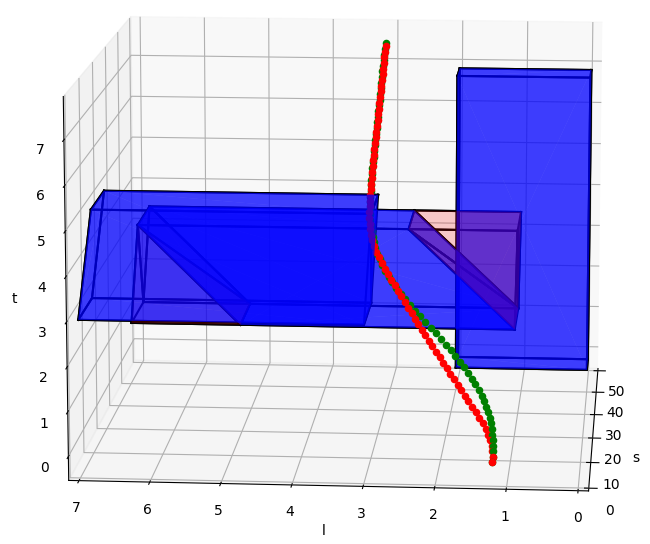
\includegraphics[width=0.32\textwidth]{figures/s1/s1_1.png}\label{fig:f8}}
    \subfloat[]{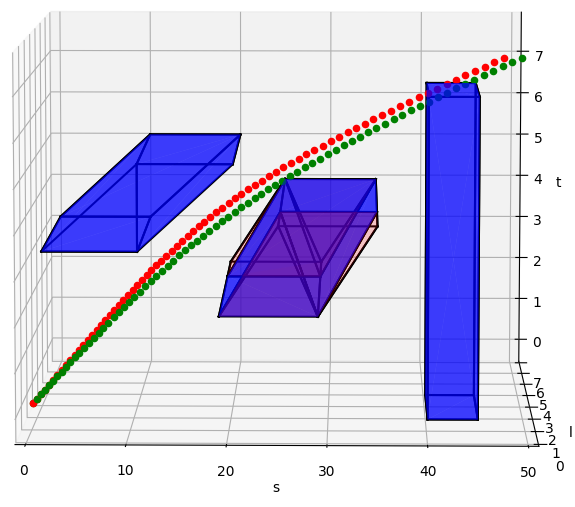
\includegraphics[width=0.32\textwidth]{figures/s1/s1_2.png}\label{fig:f9}}\\
    \textnormal{两种方法生成的轨迹（绿色为梯形，红色为长方体）}
    \subfloat[纵向加速度曲线]{
\includegraphics[width=0.32\textwidth]{figures/s1/dds.png}\label{fig:f12}}
    \subfloat[横向加速度曲线]{
\includegraphics[width=0.32\textwidth]{figures/s1/ddl.png}\label{fig:f13}}\\
    \subfloat[纵向速度曲线]{
\includegraphics[width=0.32\textwidth]{figures/s1/ds.png}\label{fig:f10}}
    \subfloat[横向速度曲线]{
\includegraphics[width=0.32\textwidth]{figures/s1/dl.png}\label{fig:f11}}
    \caption{分段 B\'{e}zier 多项式及其动力学曲线}
    \label{fig: Fig 3}
\end{figure}

图 \ref{fig:f8} 和图 \ref{fig:f9} 给出了针对图 \ref{fig:motivation} 所示场景，分别由长方体走廊（红色，\cite{ding_safe_2019}）和梯形棱柱走廊（绿色，本文方法）生成的 B\'{e}zier 曲线。从图 \ref{fig:f12} 可见，我们方法所需的最大加速度小于长方体走廊方法所需的值。图 \ref{fig:f13} 记录了两种方法的横向加速度，从中可以更清晰地看出梯形走廊的优越性。我们观察到，本文方法给出的加速度曲线更平滑，急动度较小，且最大加速度更低。我们还针对同一场景测试了两种方法的最大初始条件，以展示扩大搜索空间的效果。采用梯形走廊时，我们可以在 $a_s = 2$ \text{m/s}\textsuperscript{2}, $v_s = 10.5$ \text{m/s}, $a_l = 1.2$ \text{m/s}\textsuperscript{2}, $v_l = 2$ \text{m/s} 的条件下生成轨迹，此时纵向加速度的界为 $[-3, 2]$ \text{m/s}\textsuperscript{2}，横向加速度的界为 $[-2, 2]$\ \text{m/s}\textsuperscript{2}。而长方体走廊在上述初始条件下无法生成轨迹，只有当纵向初始速度降到 9\ m/s 时才成功。

\subsubsection{超越前方低速车辆} 我们测试规划器在两次换道（第二次变回自车原车道）中超越前方缓行车辆的表现。在分层规划方法中，这类场景通常通过将障碍物视为若干秒内的静态目标来处理，因此偏保守。%Through our experiments with our direct optimization approach, we conclud that within the comfort-optimal limits for acceleration and jerk, the planner cannot find a complete trajectory for a time horizon of $7\ s$, but was sucessful when we increased the horizon to $10\ s$.
两种走廊生成方式在纵向加速度曲线上的差异见图 \ref{fig:overtake}。显然，采用梯形走廊所生成的轨迹加速度要低得多。本场景中，前车以 $v_s = 5$\ m/s 匀速行驶，自车初始条件为 $v_s = 7$ \ m/s。

\begin{figure}[htbp]
    \centering
    \subfloat[纵向加速度]{
\includegraphics[width=0.35\textwidth]{figures/overtaking/dds.png}\label{fig:overtake_a}}\quad
    \subfloat[\textit{matplotlib} 动画]{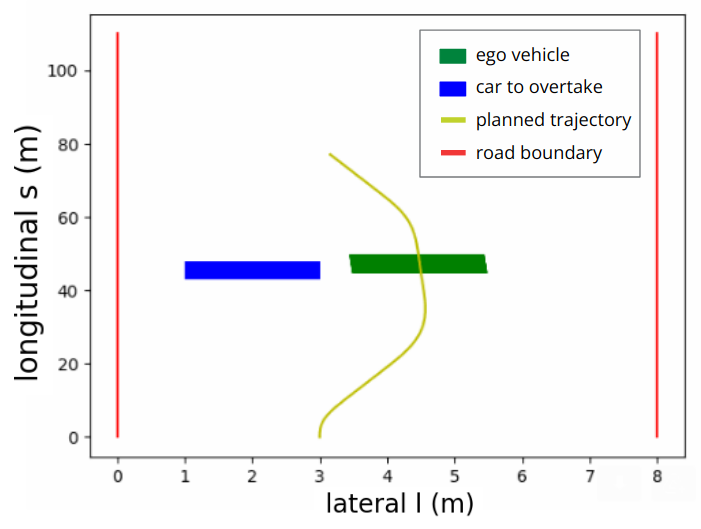
\includegraphics[width=0.23\textwidth]{figures/overtaking/matplotlib_overtake.png}\label{fig:overtake_b}}
    \caption{超车场景}
    \label{fig:overtake}
\end{figure}

\subsubsection{无保护左转}
%To verify that our proposed method can automatically adapt to different traffic configurations other than yielding and overtaking on straight roads, we choose to
%We verify our planner in an unprotected left turn scenario at an intersection.
如图 \ref{fig:f18} 所示，前方有两辆来车，若不让行则自车无法完成左转。由图 \ref{fig:f16} 可见，我们的规划器能够在满足所有安全和动力学可行性约束的前提下成功找到一条轨迹。由于自车需要对前方来车让行，我们也测试了该场景下纵向方向上的最大初始速度（$v_s = 1$\ m/s）与加速度（$a_s = 0.5$\ m/s\textsuperscript{2}）。当 A 车与 B 车之间的距离足够自车从中穿过时，我们的规划器能够找到相应的轨迹（图 \ref{fig:f17}）。该场景中，由梯形走廊带来的额外搜索空间完全没有被利用，因为穿越扩大后的搜索空间只会导致换道，而这并非期望行为。因此，两种方法所得到的轨迹完全一致并相互重合，见图 \ref{fig: Fig 5}。

\begin{figure}[htbp]
    \centering
    \subfloat[自车以蓝色表示，附带相应的参考轨迹]{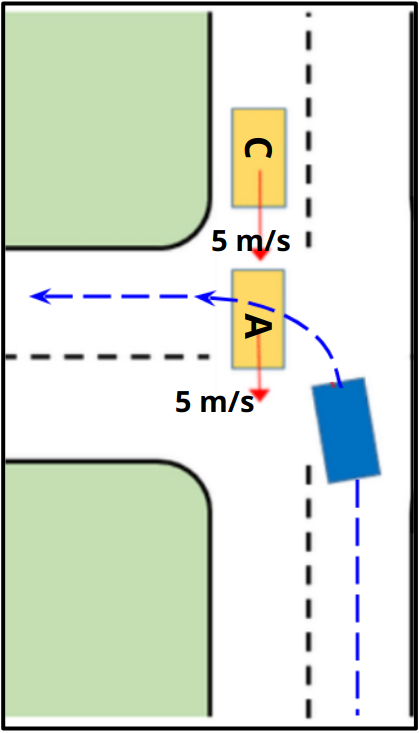
\includegraphics[width=0.32\textwidth, angle=90]{figures/left_turn/left_turn.png}\label{fig:f18}}\\
    \subfloat[]{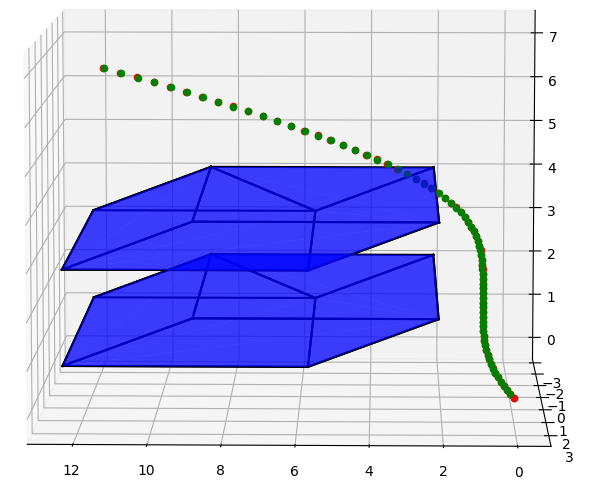
\includegraphics[width=0.32\textwidth]{figures/left_turn/s1.png}\label{fig:f16}}
    \subfloat[]{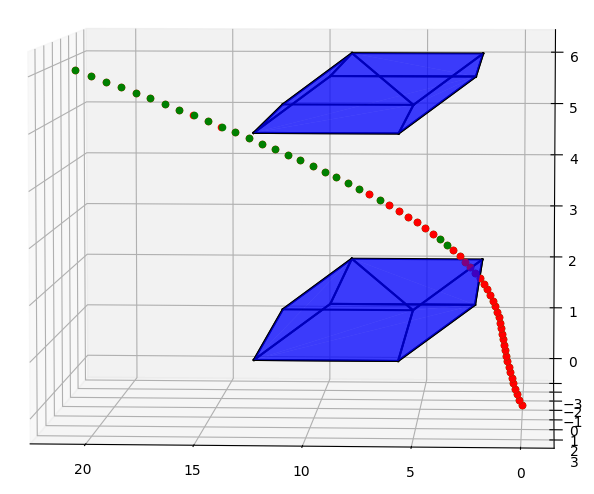
\includegraphics[width=0.32\textwidth]{figures/left_turn/s2.png}\label{fig:f17}}
    \caption{交叉口无保护左转 —— 两种走廊构造方法得到的轨迹（绿色为梯形，红色为长方体）完全相同}
    \label{fig: Fig 5}
\end{figure}

\subsection{CommonRoad 仿真}
本部分的仿真在 CommonRoad 平台上进行 \cite{commonroad}，该平台提供了用于验证运动规划算法的交互式仿真环境和非交互式真实交通环境。当自车在满足所有约束的条件下到达期望的目标区域时，认为给定场景被“求解成功”。我们在图 \ref{fig:motivation} 所示换道场景下将仿真以鸟瞰图呈现。采用本文方法所得到的结果见图 \ref{fig: Fig 6}。长方体走廊方法由于搜索空间不足，重规划失败，未能给出无碰撞轨迹，其加速度也显著偏高，参见图 \ref{fig:f12}。

\begin{figure}[htbp]
    \centering
    \subfloat[$t=0\ s$]{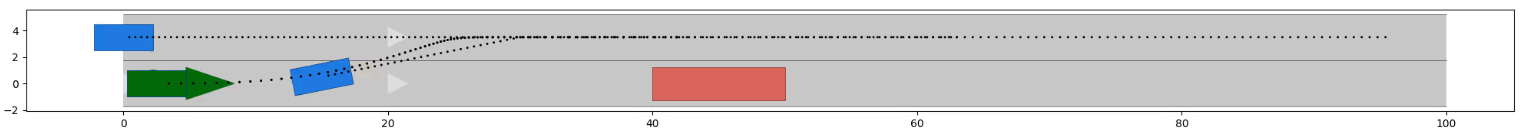
\includegraphics[width=0.55\textwidth, angle=90]{figures/commonroad/s1/t_0.png}\label{fig:c1}}\quad\quad
    \subfloat[$t=2\ s$]{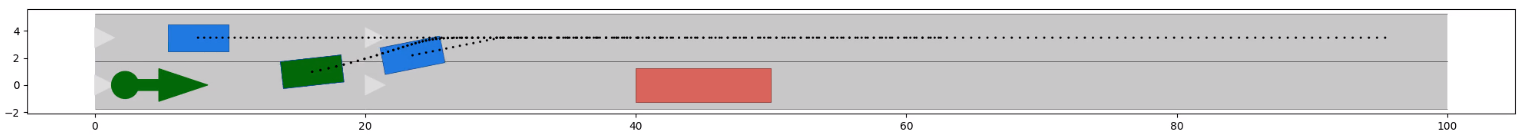
\includegraphics[width=0.55\textwidth, angle=90]{figures/commonroad/s1/t_2.png}\label{fig:c2}}\quad\quad
    \subfloat[$t=4\ s$]{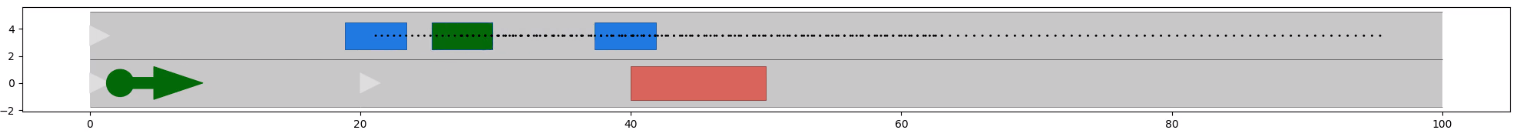
\includegraphics[width=0.55\textwidth, angle=90]{figures/commonroad/s1/t_4.png}\label{fig:c3}}\quad\quad
    \subfloat[$t=7\ s$]{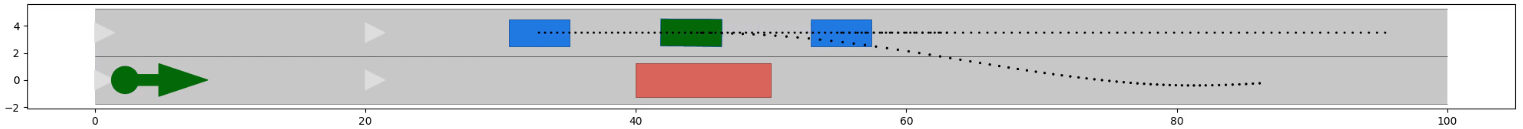
\includegraphics[width=0.55\textwidth, angle=90]{figures/commonroad/s1/t_7.png}\label{fig:c4}}\quad\quad
    \subfloat[$t=9\ s$]{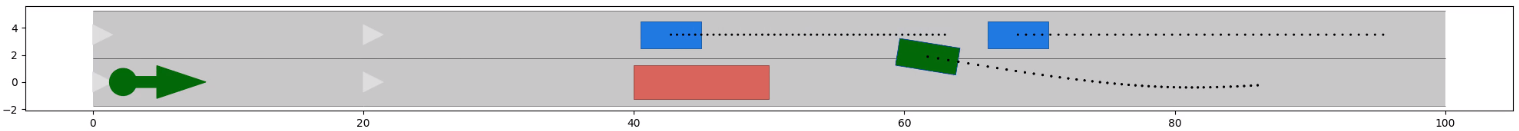
\includegraphics[width=0.55\textwidth, angle=90]{figures/commonroad/s1/t_9.png}\label{fig:c5}}\quad\quad
    \subfloat[$t=12\ s$]{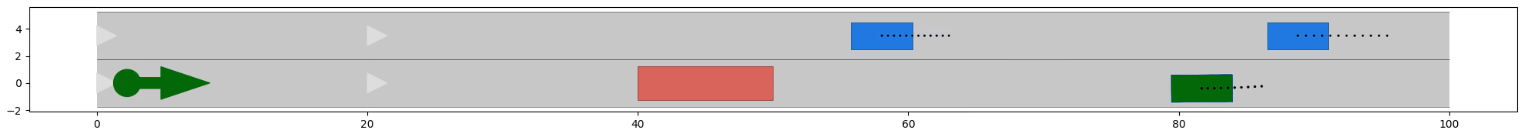
\includegraphics[width=0.55\textwidth, angle=90]{figures/commonroad/s1/t_12.png}\label{fig:c6}}
    \caption{针对“因道路施工并入另一车道”场景的 CommonRoad 仿真。自车（初始位置由绿色箭头标示）以绿色显示，其他车辆以蓝色显示，施工区域（静态障碍物）以红色显示。}
    \label{fig: Fig 6}
\end{figure}

\section{结论}

本文提出一种新的凸化算法，用于在 $S-L-T$ 空间中生成安全走廊。我们表明，所提出的梯形棱柱形走廊相较于已有的长方体走廊方法扩大了解空间。我们给出梯形走廊中控制点的充分条件，以在理论上保证由 B\'{e}zier 多项式表示的轨迹的安全性。最后，我们将轨迹优化建模为二次规划问题。数值仿真与 CommonRoad 仿真结果表明，所提方法在最优性与低失败率方面均更为优越。未来工作包括采用基于动态规划的方法，在 $S-L-T$ 空间中生成舒适最优的参考轨迹。



%%%%%%%%%%%%%%%%%%%%%%%%%%%%%%%%%%%%%%%%%%%%%%%%%%%%%%%%%%%%%%%%%%%%%%%%%%%%%%%%

%\nocite{*}  % Without this, cite articles in text using \cite{...}
\printbibliography

\end{document}




